\documentclass[12pt,letterpaper,english]{report}
%\usepackage[T1]{fontenc}
%\usepackage[latin1]{inputenc}

\setcounter{secnumdepth}{3}
\setcounter{tocdepth}{2}
\usepackage{float}
\usepackage{amsmath}
\usepackage{graphicx}
\usepackage{setspace}
\usepackage{amssymb}
\usepackage{lscape}
\usepackage{cite}
\usepackage{indentfirst}
\usepackage{babel}
\usepackage{caption}
\usepackage{subcaption}
\usepackage{listings}    

\renewcommand{\topfraction}{0.9}
\renewcommand{\bottomfraction}{0.9}
\renewcommand{\textfraction}{0.1}
\renewcommand{\floatpagefraction}{0.75}

% Custom packages
%\usepackage[first]{datestamp}   % Datestamp on first page of each chapter
\usepackage[fancyhdr]{KUThesis} % Thesis style
\usepackage{KUThesis} % Thesis style
\usepackage{KULogo}             % The University of Kansas seal
\usepackage{color}
\def\headrulehook{\color[rgb]{0.20,0.46,0.81}}        % Color the header rule

%===== page layout

\setlength{\topmargin}{0.0in}
\setlength{\topskip}{0.25in}    % between header and text
\setlength{\textheight}{8.5in} % height of main text
\setlength{\textwidth}{5.75in}    % width of text
\setlength{\oddsidemargin}{0.5in} % odd page left margin
\setlength{\evensidemargin}{0.5in} % even page left margin

\makeatletter

 \newcommand {\Sigline}[1] {\noindent \begin{minipage}{3in} 
 \rule {3 in} {0.4 pt} \\ 
			#1
 \end {minipage}
 \hfill 
 \begin{minipage} {1.5 in} 
 \rule {1.5 in} {0.4 pt} \\
 
 
 \end{minipage}}

\makeatother

\title{Biometric Analysis of Ear Recognition using Shallow and Deep Techniques}
\author{Soumyajit Sarkar}
\date{\today}

\begin{document}

\organization{%
%  \\[0.2in]
%  KUSeal {!}{1.2in}\\    % KU crest
%  \\[0.2in]
  \\[1.6in]
  Submitted to the Department of Electrical Engineering \&\\
  Computer Science and the Faculty of the Graduate School\\
  of the University of Kansas in partial fulfillment of\\
  the requirements for the degree of Master's of Science}
  \note{%
  %{\color[rgb]{0.20,0.46,0.81} \hrule height 0.4ex}
  \vskip 2ex
  \copyright\ \the\year\ Soumyajit Sarkar
}

\maketitle
%===== Justification, spacing for the main text
\raggedbottom
\onehalfspacing

\pagenumbering{roman}
\pagestyle{plain}
\newpage
\addcontentsline{toc}{chapter}{Acceptance Page}
\begin{center}
The Thesis Committee for Soumyajit Sarkar certifies\\
That this is the approved version of the following thesis:
\vskip 10ex
\textbf{Biometric Analysis of Ear Recognition using Shallow and Deep Techniques}


\vskip 10ex
Committee:
\vskip 10ex
\Labelline{Chairperson}
\vskip 6ex
\Labelline{}
\vskip 6ex
\Labelline{}
\vskip 6ex

\end{center}

\newpage
%\begin{abstract}
\chapter*{Abstract} \addcontentsline{toc}{chapter}{Abstract}f
This is the abstract
%\end{abstract}


\newpage
\tableofcontents
\listoffigures
\listoftables

\newpage
%\pagestyle{plain}
\pagenumbering{arabic}
\setcounter{page}{1}
\doublespacing

\chapter{Introduction} \label{sec:intro} Biometric authentication of people based on various anatomical characteristics, like eye, ear, face, iris, and fingerprint have attracted lots of attention during the past few decades, and some of these techniques have already been successfully applied for recognition and authentication. However, many systems are not very robust and may fail to work under certain conditions. Biometric ear recognition is a relatively new technique that may surpass the existing systems due to several significant reasons. For example, the acquisition of ear images is relatively easy and, unlike iris, can be captured without the co-operation of individuals \cite{pflug2012ear}

Human ear contains rich and stable features which are more reliable than face fea- tures, as the structure of the ear is not subject to change with age. It has also been found out that no two ears are exactly the same even for identical twins \cite{abaza}. The detailed structure of ear is not only very unique but also permanent, since the shape of a human ear never shows drastic changes over the course of life. The research on ear identification was first conducted by Bertillon, a French criminologist, in 1890. The process was refined by American police officer, Iannarelli [20], who divided the ear based on various distinctive features of seven parts: i.e. helix, concha, antihelix, crux of helix, inter- tragic notch, tragus, and antitragus \cite{tariq}.

One of the first ear recognition systems is Iannarelli's system developed originally in 1949. This manual system has basically 12 measurements.Each photograph of the ear is aligned such that the lower tip of a standardized vertical guide on the development easel touches the upper flesh line of the cocha area, while the upper tip touches the outline of the antitragus. Then the crus of helix is detected and used as a center point. Vertical, horizontal, diag- onal, and anti-diagonal lines are drawn from that center point to intersect the internal and external curves on the surface of the pinna. The 12 measurements are derived from these intersections and used to represent the ear \cite{abaza}.

Fields et al. [1960] made an attempt to identify newborn babies in hospitals. They visually assessed 206 sets of ear photographs, and concluded that the morphological constancy of the ear can be used to establish the identity of the newborn.

The human ear starts to develop between the fifth and seventh weeks of pregnancy.At this stage, the embryo’s face takes on more definition as a mouth perforation, nostrils, and ear indentations become visible. Though there is still disagreement as to the precise embryology of the external ear , the ear development during pregnancy is listed below:

 
1) The embryo develops initial clusters of embryonic cells that serve as the foundation from which a body part or organ develops. Two of these clusters, termed the first and second pharyngeal arches, form six tissue elevations called auricular hillocks during the fifth week of development. 

2) In the seventh week,the auricular hillocks begin to enlarge,differentiate,and fuse, producing the final shape of the ear, which is gradually translocated from the side of the neck to a more cranial and lateral site. By the ninth week, the morphology of the hillocks is recognizable as a human ear.

Currently there is no such biometric system which is being used commercially for automatic identification of verification of the ear biometric.

Here, we propose to use two scale and rotation invariant feature detectors, i.e. SIFT (scale invariant feature transform) and SURF (speed up robust features), for ear recognition. Both SIFT and SURF extract specific interest points from an image and generate descriptors for the feature points to a form a reliable matching results.\\
%Path in Mac Format
\begin{figure}[t]
	\DeclareGraphicsExtensions{.pdf,.png,.jpg}
	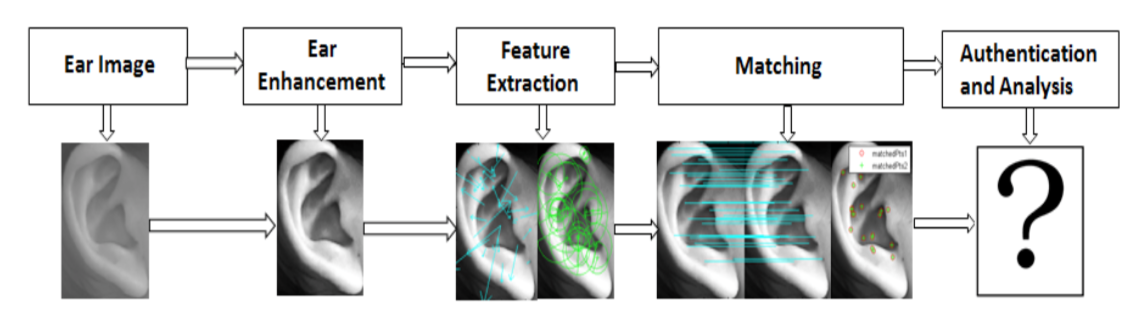
\includegraphics[width=\textwidth]{Figures/Figure1}
	\caption{The pipeline of the proposed Ear Recognition System}
	\label{fig:Figure1}
\end{figure}
Extensive experiments have been carried out on two different sets of databases to evaluate their performance with respect to various rotations and scales. One of the most important feature of ear images is its easiness in acquisition, however, the acquired images may be in different scales, rotations, and illumination. The scale and rotation invariant property of the SIFT and SURF algorithms makes them perfect for ear authentication under various circumstances.

 A new concept in the field of machine learning and computer vision has come up which has surpassed the traditional object recognition methods. This new approach is called deep learning. Deep Learning is a branch of Machine Learning which has multiple levels of representations and abstractions. It is basically a rebranding of the term Artificial Neural Networks. Deep Learning algorithms have already been applied in Apple's Siri, Google's Streetview etc. 
 
 The reason behind the rise of ear biometrics is that the structure of the ear is not only unique but also permanent. Since the acquisition of ear images does not require a person's co-operation, due to these advantages the interest in ear recognition research has grown significantly in the past few years. One of the most important challenges in ear biometrics is occlusion and pose variation, in contrast to the face, the ear is sometimes partially occluded by hair, ear-rings, headphones. Robustness against occlusions have been addressed in previous publications \cite{pflug2012ear}. But no studies have been covered on the effect of certain types of occlusion like hair or earrings. 
 
 Pose variations has also been another challenge in this domain where the subject's ear is never straight and is moving all the time when the images are captured from different angles. Thus scalability and pose remains a concern. In this project, details on pose variations and scales have been provided and analysis has also been done to see how it affects the performance of the system.
 
 The symmetry of the right and left ear has not been understood yet.The studies of Iannarelli indicates that some characteristics of the outer ear can be inherited and another factor is ageing. These assumptions does not have a proof since ear recognition is still a relatively new field of research. Lighting condtitions, pose variations till remain a great challenge to the performance of the biometric systems. Though good databases are available, it is still difficult to get better performances as most of the databases follow a specific standard and they are taken under the same light and pose variations.
 
 

The rest  is organized as follows. Some background and related research are discussed in Section 3; The proposed method is presented in details in Section 4; Some experimental results and analysis are given in Section 4.5; Ongoing and future work is being described in Section 5 with Conclusion in Section 6.
\chapter{Statement of the Problem}
\label{sec:problem}

\section{Types of Biometrics} Biometrics has been an active field of research over the last decade. The reason behind their success is that biometric characteristics are universal, unique and permanent. Unlike other forms of authentication such as passwords or identification cards which can be stolen or faked easily.

There are many kinds of biometrics which can be used for authentication purposes. Among them the prominent being, Face, Ear, Palm, Fingerprint\cite{fingerprint}, Iris and others which are frequently being used these days in day to day life to authenticate an individual. Another reason biometrics have been used these days are due to terrorist activities and other fraudulent ways in which people impersonate themselves which are harder to catch. These days biometrics are used everywhere from Airports to ATMs to secured entry to corporate offices where checking the identity of an identity of an individual is mandatory before access is given. It helps to strengthen the security of an organization or country potential threat. As mentioned above, the different types of biometrics, different biometrics have different purposes and importance. The most popular being face recognition which is being used everywhere to authenticate people, the only disadvantage being the change in facial expression and with age the face changes upto a certain extent which makes it difficult to recognize and authenticate. Fingerprint is also being used in almost any high priority zone nowadays to authenticate and is very successful but it requires complete co-operation of an individual in order to authenticate them. The same problem happens with iris authentication where it becomes very difficult to extract the iris image to match and authenticate. 

Ear authentication comes to the rescue in such a situation due to many reasons. The primary being the stability in the human ear structure and ear images can easily be captured without the co-operation of an individual. Each ear is unique, so any side image of an individual is enough in order to authenticate a person.

\section{Purpose of Biometric Ear Recognition} 

Ear authentication and recognition is being considered as one of the most innovative processes as of today. The human ear can be divided into six main parts: Outer helix,
the antihelix, the lobe, the tragus, the antitragus and the concha. The shape of the outer ear evolves during the embryonic state from six growth nodules. The structure is completely random, the randomness can be observed by comparing the left and right ear of the same person - thus they are not symmetric. French criminologist Alphonse Bertillon was the first to be aware of ear to be used for human identification purposes. His work was carried on by Alfred Ianarelli whoc collected 10,000 ear images and determined 12 characteristics needed to identify a person. He also conducted studies on twins and triplets thereby discovering that ears are unique even among genetically identical persons \cite{pflug2012ear}. The different parts of the ear are shown in Figure \ref{fig:Figure2}

\begin{figure}[t]
	\DeclareGraphicsExtensions{.pdf,.png,.jpg}
	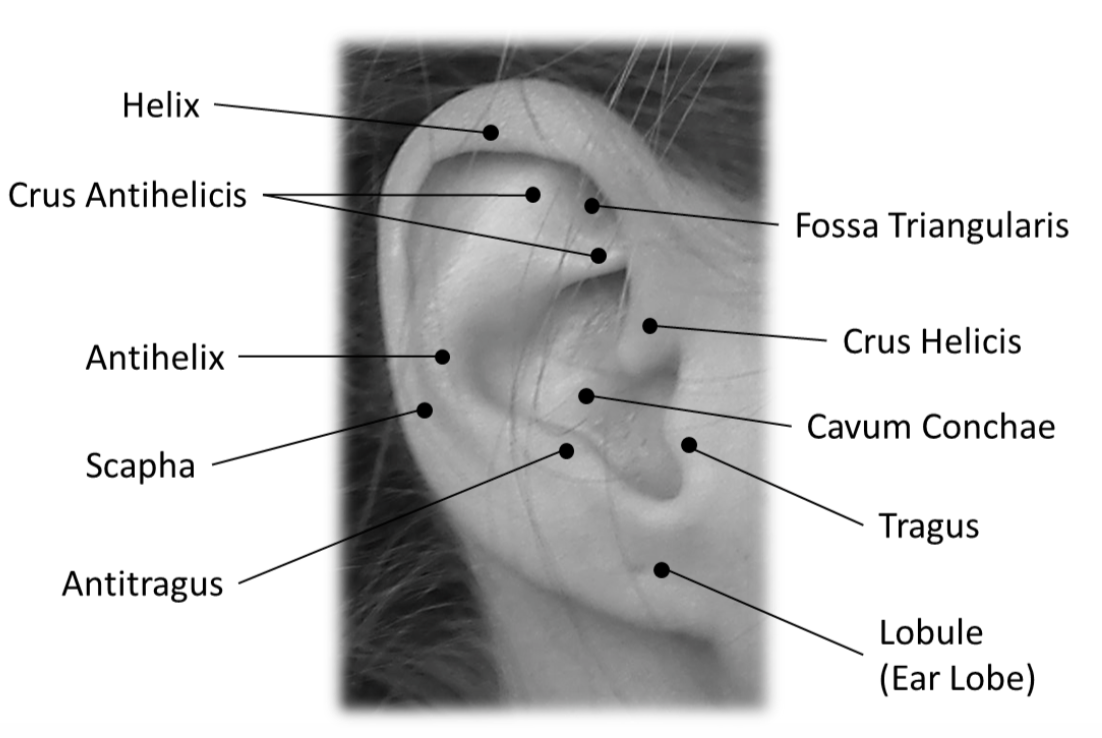
\includegraphics[width=\textwidth]{Figures/Figure2}
	\caption{Characteristics of Human Ear\cite{pflug2012ear}} 
	\label{fig:Figure2}
\end{figure}

The uniqueness of the ear has been accepted to be true based on empirical results, the underlying scientific basis of ear individuality has not been formally established. As a result, the validity of ear evidences has been challenged in several court cases. In response to a U.S Court Ruling, a large scale study involving 10,000 subjects has been proposed to determine the variability of the ear from the entire dataset. In 1906, Imhofer studied a set of 500 ears and noted that based on 4 features - he could clearly distinguish between ears. In 1989, Iannarelli\cite{Iannarelli} examined the difference in ear structures between fraternal and identical twins, it was found that despite having the same ear structures, they were still clearly distinguishable.

In 2000, Burge and Burger\cite{burger} presented a study of the uniqueness of human ear by using Iannarelli's features, they assumed an average standard deviation in the population of 4 units, the 12 measurements provided a space with 4\textsuperscript{12} variation which is less than 17 million distinct points. Purkait and Singh \cite{purkait} in 2008, presented a preliminary study to test the individuality of human ear patterns. They manually extracted 12 inter-landmark linear distances from a set of 700 male and female individuals. They found that this 12-dimensional feature space could clearly distinguish more than 99.9{\%} of ear pairs, where very few pairs had distances which fell below the safe distinction limit.

The typical ear biometric system can be viewed as a system where an input image can be reduced to a set of features that is used to compare with the features of other images to determine its identity. The salient features of a classical ear recognition system are\cite{abaza} 

\begin{enumerate}
\item Ear Detection/ Segmentation - The first stage which is used to localize the position of the ear in the image.
\item Ear Normalization and Enhancement - The size of the ear image is normalized for standardization and enhanced using standard image processing techniques in order for more features to be extracted.
\item Feature Extraction - Feature extraction refers to a process in which the ear image is being reduced to a mathematical model called a feature vector to get information.
\item Matching Features - The features extracted are then compared to the features that are extracted earlier and stored in the database to find a match.
\item Decision - Matching scores are generated by the model used to train the features to give a decision of whether the image is matched or not.
\end{enumerate}



\section{Contributions of this Project} The main goal of this work is to develop
shallow and deep techniques to extract efficient features from a set of ear images in order to authenticate a human being. A thorough comparison of two traditional techniques called SIFT(Scale-Invariant Feature Transform) \cite{sift1} \cite{sift2} and SURF(Speed-up of Robust Features have been provided) \cite{surf}, this project is a continuation of the work done by Sarkar et al \cite{sarkar}. Since the extracted features are hand-crafted, there is quite a good amount of false matching and thus it may affect the true performance of the whole process. Outlier detection is a way in Computer Vision by which several false matches can be eliminated in order to get a proper result. 

\chapter{Background}
\label{sec:back}

Human ears start to develop between fifth and seventh weeks of pregnancy. At this stage, the embryo face takes on more definition as mouth perforation, nostrils and ear indentations become visible. Forensic science literature reports that ear growth after the first four months of birth is highly linear [20]. The rate of stretching is five times greater than normal during the period from 4 months to the age of 8, after which, it is constant until the age of seventy when it again increases. Thus it can be said that ear remains almost unchanged during a substantial period of 62 years and, thus, it is one of the strong points of considering ear for biometric authentication.

Haar-based methods have given fairly better results for face detection as it is robust and fast. The different types of ear recognition systems include those of intensity-based, force-field based, 2D curves geometry, wavelet transformation, Gabor filters, SIFT, and 3D features. The force-field transforms gained popularity due to its uniqueness and efficiency [22]. Similar methods have also been implemented on other kinds of ear recognition systems [8][10].

Deep Methods have already come up and showing good performances on other face recognition systems which shows that it can also be applied to ear recognition systems. Hand-crafted feature detectors have not been able to work properly and are not robust, so deep features have been extracted to improve upon the performance. But one of the few drawbacks about deep learning is that it needs a large amount of data to train the model. There are not many ear databases that are too big but an attempt has been made to apply deep learning on a small scale database and analyze the results.

\chapter{Initial Shallow Design}
\label{sec:design}

\section{Traditional Approach} The initial scheduler in
the HybridThreads system used a simple FIFO scheduling mechanism that was
internal to the Thread Manager (TM) \cite{Andrews:2004wu}.  The add\_thread
system call would be routed to the Thread Manager and the TM would then insert
the thread into a singly-linked FIFO ready-to-run queue.  The main problem with
this scheduling structure is that the ready-to-run queue was built in to the
Thread Manager's attribute structures used for data storage for thread
management status.  This means that thread management (allocation, creation,
and control) and thread scheduling (ready-to-run queue management, and
scheduling decisions) activities could not occur in parallel.  Additionally,
any changes in scheduling mechanisms and scheduling data arrangement would also
affect the management mechanisms, and vice-versa, so maintenance of the
management and scheduling services would be difficult, cumbersome, and
error-prone.

Both the thread management and thread scheduling mechanisms would have to be
modified if either were to be extended in their functionality or data storage
requirements.  The scheduling mechanism was going to be upgraded to allow for
priority scheduling and eventually would have to handle the scheduling of both
SW and HW threads, so it was decided to make the scheduler a separate IP module
that would have its own interface to the HybridThreads system bus.  Many thread
management operations result in the invocation of scheduling operations, so
essentially the TM uses the scheduler module as a coprocessor for any and all
scheduling operations.  Many of these coprocessor operations can only occur as
a result of a management operation so the TM will always be the "caller" in
these cases.  This, in conjunction with the scheduler becoming a separate
module, means that all outgoing operations from the TM to the scheduler will
result in a bus operation; however if the TM is using the scheduler to complete
a management operation, then the bus will already be locked by the caller of
the TM operation.  This meant that a special interface must be
created between the TM and the new scheduler module to allow access to
scheduling operations while the system bus was locked.  Additionally, since
other scheduler specific operations are not ever called as the result of a thread
management operation, then these scheduling operations can be called via the
new interface used to attach the independent scheduler module to the
HybridThreads system bus.

The TMcom interface is a dedicated hardware interface between the scheduler
module and the TM that consists of a total of seven control and data signals as
well as access to a read-only interface (B-port) of the TM's Block RAM (BRAM).
The data signals include \texttt{Next\_Thread\_ID},
\texttt{Current\_Thread\_ID}, and \texttt{Thread\_ID\_2\_Sched}.  The
\texttt{Next\_Thread\_ID} signal represents the identifier of the thread chosen
to run next on the CPU.  This signal is writable by the scheduler module and
readable by the TM.  The \texttt{Current\_Thread\_ID} signal represents the
identifier of the thread that is currently running on the CPU (PowerPC 405).
This signal is readable by the scheduler module and writable by the TM.  The
\texttt{Thread\_ID\_2\_Sched} signal contains the identifier of the thread that
is being added to the ready-to-run queue by the TM.  This signal is readable by
the scheduler and writable by the TM.  The control signals include
\texttt{Next\_Thread\_Valid}, \texttt{Dequeue\_Request},
\texttt{Enqueue\_Request}, and \texttt{Enqueue\_Busy}.  The
\texttt{Next\_Thread\_Valid} signal represents whether or not that the
scheduling decision available from the scheduler module on the
\texttt{Next\_Thread\_ID} signal is valid or not (Valid = 1, Invalid = 0).
This signal is writable by the scheduler module and readable by the TM.  The
\texttt{Dequeue\_Request} signal is used by the TM to request the scheduler
module to perform a dequeue operation of the thread whose identifier is on the
\texttt{Next\_Thread\_ID} signal.  This signal is readable by the scheduler
module and writable by the TM.  The \texttt{Enqueue\_Request} signal is used by
the TM to request the scheduler module to perform an enqueue operation of the
thread whose identifier is on the \texttt{Thread\_ID\_2\_Sched} signal.  This
signal is readable by the scheduler module and writable by the TM.  The
\texttt{Enqueue\_Busy} signal represents whether or not the scheduler is
currently busy performing an enqueue operation (Busy = 1, Not Busy = 0).  This
signal is writable by the scheduler module and readable by the TM.  The B-Port
interface to the TM's BRAM allows the scheduler module to query thread
management information in order to perform error-checking that concerns the
parent-child relationships of threads that the TM's data structures hold.  The
purpose of the TMcom interface is to allow the TM to request scheduling
operations as a result of thread management operations whose side-effects alter
the scheduling status of the system (i.e. the status of the ready-to-run
queue).  The operations available through the TMcom interface can be seen in table
\ref{tab:commands1}.

\begin{table}
\caption{\label{tab:commands1}Command Set of Scheduler Module, Build 1}
\centering
\begin{tabular}{llp{3.0in}}
\hline
\multicolumn{1}{c}{\textbf{Type}} &
\multicolumn{1}{c}{\textbf{Name}} &
\multicolumn{1}{c}{\textbf{Actions}} \\
\hline
TMcom	&	Enqueue				& Schedules a thread\\
TMcom	&	Dequeue				& Removes a thread from the ready-to-run queue	\\
BUScom	&	Get\_Entry     		& Returns a thread's table attribute entry		\\
BUScom	&	Toggle\_Preemption	& Toggle preemption interrupt on/off	\\
BUScom	&	Get\_Entry     		& Returns a thread's table attribute entry (for debug use)		\\
BUScom	&	Get\_Priority		& Returns the priority-level of a thread	\\
BUScom	&	Set\_Priority		& Sets the priority-level of a thread\\
BUScom	&	Set\_Default\_Priority		& Sets the priority-level of a thread (no error-checking)\\
\hline
\end{tabular}
\end{table}


\section{SIFT and SURF Descriptor}
\label{sec:build2}

\textbf{Speed up Robust Features(SURF) - } SURF is a high performance, fast scale and rotation invariant point detector and descriptor.The task of finding point correspondences between two images of the same scene or object is part of many computer vision applications. Image registration, camera calibration, object recognition, and image retrieval are just a few.The search for discrete image point correspondences can be divided into three main steps. First, ‘interest points’ are selected at distinctive locations in the image, such as corners, blobs, and T-junctions. The most valuable prop- erty of an interest point detector is its repeatability. The repeatability expresses the reliability of a detector for find- ing the same physical interest points under different viewing conditions. Next, the neighbourhood of every interest point is represented by a feature vector. This descriptor has to be distinctive and at the same time robust to noise, de- tection displacements and geometric and photometric deformations. Finally, the descriptor vectors are matched be- tween different images. The matching is based on a distance between the vectors, e.g. the Mahalanobis or Euclidean distance. The dimension of the descriptor has a direct impact on the time this takes, and less dimensions are desirable for fast interest point matching. However, lower dimensional feature vectors are in general less distinctive than their high-dimensional counterparts.
It has been our goal to develop both a detector and de- scriptor that, in comparison to the state-of-the-art, are fast to compute while not sacrificing performance. In order to succeed, one has to strike a balance between the above requirements like simplifying the detection scheme while keeping it accurate, and reducing the descriptor’s size while keeping it sufficiently distinctive.
 It outperforms previously proposed schemes with respect to repeatability, distinctiveness and robustness [9]. The detector is based on the Hessian matrix and uses a very basic Laplacian-based detector, called difference of Gaussian (DoG). The implementation of SURF can be divided into three main steps. First, interest points are selected at distinctive locations in the image, such as corners, blobs, and T-junctions. Then, the neighborhood of every interest point is represented by a feature vector. This descriptor has to be distinctive and robust to noise, detection errors, and geometric and photometric deformations. Finally, the descriptor vectors are matched between different images. When working with local features, the issue that needs to be settled is the required level of invariance. Here the rotation and scale invariant descriptors seem to offer a good compromise between feature complexity and robustness to commonly occurring deformations, skew, anisotropic scaling, and perspective effects [9].

Given a point in an Image, the Hessian matrix is as follows:

\[
H(x,\sigma) =  
	\begin{bmatrix}
		L_{xx}(x,\sigma) &  L_{xy}(x,\sigma)\\
		L_{xy}(x,\sigma) &  L_{yy}(x,\sigma)
	\end{bmatrix}
\]

where $L_{xx}(x,\sigma)$ is the convolution of the gaussian second order derivative 
$\frac{d^2}{dy^2}g(\sigma)$ at the point. This method leads to a novel detection, description and subsequent matching steps. Using relative strengths and orientations of gradient reduces the effect of photometric changes. Figure \ref{fig:Figure9} shows the detection results with respect to rotation and scale change. As shown in Section 4, it has been found that though SURF is rotation invariant, its performance in matching, i.e. matching score, decreases sharply when the im- ages are rotated or scaled. The SURF features are not stable over various rotation angles and scale changes.
\\ 
\begin{figure}
	\DeclareGraphicsExtensions{.pdf,.png,.jpg}
	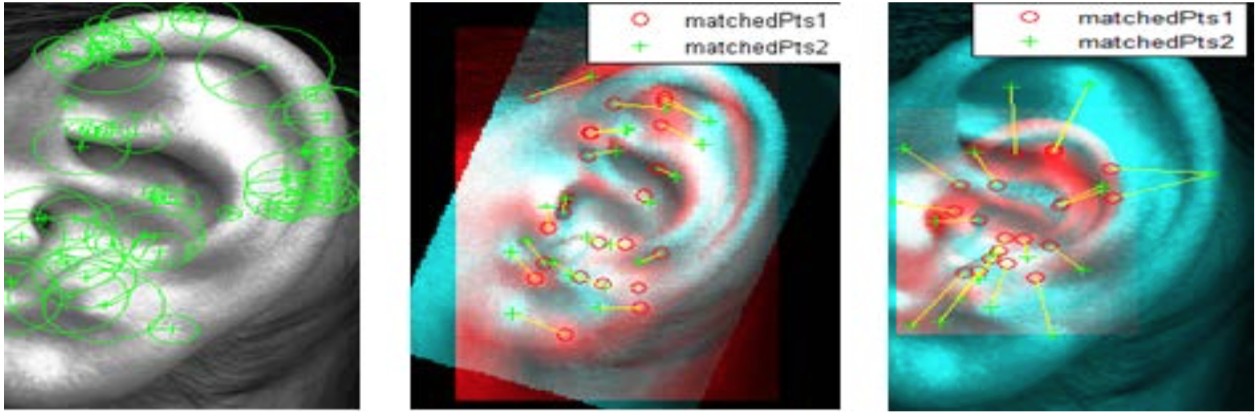
\includegraphics[width=\textwidth]{Figures/Figure9}
	\caption{The detected SURF features (left) and matching result under rotation (middle) and scale change (right)}
	\label{fig:Figure9}
\end{figure}

\textbf{Scale Invariant Feature Transform(SIFT) - } The SIFT features are invariant to image scaling and rotation and shown to provide robust matching across a substantial range of affine distortion, change in 3D viewpoint, addition of noise, and change in illumination. Image matching is a fundamental aspect of many problems in computer vision, including object or scene recognition, solving for 3D structure from multiple images, stereo correspondence, and motion tracking. This paper describes image features that have many properties that make them suitable for matching differing images of an object or scene. The features are invariant to image scaling and rotation, and partially invariant to change in illumination and 3D camera viewpoint. They are well localized in both the spatial and frequency domains, reducing the probability of disruption by occlusion, clutter, or noise. Large numbers of features can be extracted from typical images with efficient algorithms. In addition, the features are highly distinctive, which allows a single feature to be correctly matched with high probability against a large database of features, providing a basis for object and scene recognition.
The cost of extracting these features is minimized by taking a cascade filtering approach, in which the more expensive operations are applied only at locations that pass an initial test. 3D-SIFT \cite{3dsift} algorithms have also been researched upon to get a better understanding for 3-dimensional object feature extraction and matching.

 The computation stages of SIFT are as follows: \\
Step 1. Scale space extrema detection: The first step is to construct a Gaussian scale over all the locations. It is implemented efficiently by using a difference of Gaussian (DoG) to identify potential interest points. The 2D Gaussian operator G(x,y,σ) is convolved with the input image \textit{I(x,y)}:
\begin{center}
	$L(x,y,\sigma) = G(x,y,\sigma) * I(x,y)$
\end{center}
where the  DoG images are obtained by subtracting the subsequent scales in each octave.
\begin{center}
	$G(x,y,\sigma) = L(x,y,k\sigma) - L(x,y,\sigma)$
\end{center}

Step 2. Accurate keypoint localization: Once a keypoint has been detected, a detailed model is fitted to determine its location and scale. The keypoints are selected based on measures of their stability. Further details can be found in \cite{alonso2009iris}. 

Step 3. Orientation assignment: One or more orientations are assigned to each key- point location based on local image gradient directions. All future operations are per- formed on image data that has been transformed relative to the assigned orientation, scale, and location for each feature.

Step 4. Keypoint descriptor: The local image gradients are measured at selected scale in the region around each keypoint. They are transformed into a certain representation that allows for significant levels of local shape distortion and shape illumination.

Figure \ref{fig:test4} shows an evaluation of the SIFT detector. It is evident the SIFT keypoints are very stable when the images are rotated and scaled. The scaling results are much better compared to the rotation results in our experiments.
\begin{figure}
\centering
\begin{subfigure}{.5\textwidth}
  \centering
  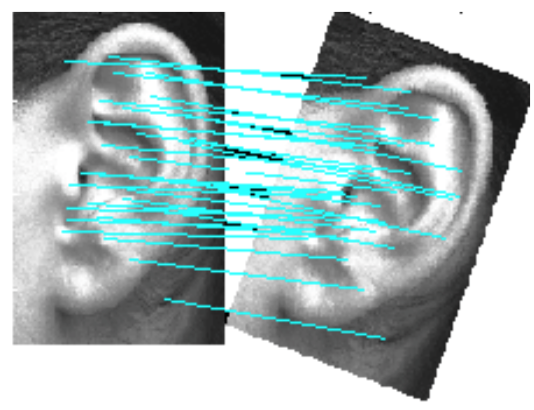
\includegraphics[width=.5\linewidth]{Figures/Figure11}
  \label{fig:sub11}
\end{subfigure}%
\begin{subfigure}{.5\textwidth}
  \centering
  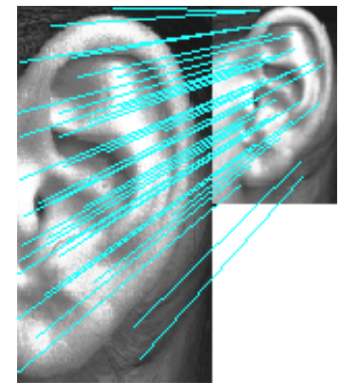
\includegraphics[width=.5\linewidth]{Figures/Figure12}
  \label{fig:sub12}
\end{subfigure}
\caption{The matching results of SIFT detectors under rotation (left) and scale change (right)}
\label{fig:test4}
\end{figure}

\section{False Match Removal} 

Fundamental Matrix estimation from two views plays an important role in 3D Computer Vision. It contains all geometric information about the relative transformation between images. The estimation is actually based on solving a homogeneous linear system where each linear equation is formed by a pair of correspondence feature points. A large number of robust estimation approaches have been proposed to alleviate the influence of outliers to the fundamental matrix estimation. Some of them include the M-estimator method which reduces the effect of outliers by by applying weight functions to transform the problem to a weighted least squares problem. However, the approach needs a good initial estimation and only works under low percentages of outliers.This method is very time-consuming.

Random Sample Consensus or RANSAC[RANSAC Paper] is a very popular algorithm for Fundamental Matrix Estimation. It uses minimal points set to estimate an initial guess and then the confidence of the estimation is established by testing each point correspondence against the model with an inlier set, which is determined by choosing points that have error below a given threshold. After that, a new fundamental matrix is estimated by the inlier set, thus iteratively the RANSAC algorithm attempts to find a solution that maximizes the amount of inlier set.

Re-projection error is adopted in this approach[Ming Paper] rather than the widely used algebraic error for confidence evaluation purposes.  An assumption is made of gaussian noise present in each image and the reprojection error of point correspondence can be described by a chi-square distribution. The outliers are eliminated by a 3-sigma principle.

For Robust Fundamental Matrix Estimation, an Eight-point linear algorithm is used, where  estimation from a set of point correspondences between two images is performed. Given a set of two images \textit{I} and \textit{I'}, suppose $x_i \in \textit{I}$ and $x'_{i} \in \textit{I'} $ are a pair of corresponding homogeneous points between the two images, The fundamental matrix \textbf{F} satisfies the following equation:

\begin{center}
	$x^{'T}_i \textbf{F} x_i  = 0$
\end{center}

where the fundamental matrix is a 3 X 3 homogeneous matrix defined up to scale. Each pair of point correspondence yield one linear constraint for the entries of \textbf{F}. Thus the estimation of the fundamental matrix can be done with eight point pairs. When more correspondences are available, the fundamental matrix can be estimated via least squares. 

To evaluate the error for each pair of point correspondence, a perspective 3D reprojection of all the corresponding points can be obtained via triangulations. The reconstructed 3D points can be reprojected back to the two images via the camera matrices. let us suppose $\mathbf{\hat{x}}_i$ and $\mathbf{\hat{x}}'_i$ are the reprojected images of point $i$, the 2D reprojection error of the corresponding point is defined as
\begin{equation}
e_{r}(i) = \frac{1}{2} \sum \|\mathbf{x}_i-\mathbf{\hat{x}}_i\|^2_F + \|\mathbf{x}'_i-\mathbf{\hat{x}}'^2_i\|_F, \;\;\;s.t.\;\;\; 
\mathbf{\hat{x}}'^T_i \mathbf{F} \mathbf{\hat{x}}_i=0 \;\;\; \forall i
\end{equation}


The 2D reprojection error is proven to be more superior to other geometric errors. Optimal triangulation is a linear triangulation method which converts the least-square function to a one parameter function and finds a global optimal solution.

Now, for the strategy for outlier detection, it is being assumed that the image noise is modeled by Gaussian distribution. Through intensive simulations, it is being found that the reprojection errors of outliers are usually greatly larger than those of inliers. As a result, these outliers can be identified using 3-sigma principle. Points with reprojection errors larger than the triple variance of all the reprojection error can be classified as outliers. Based on robust statistics [15:Ming Paper], we can obtain a robust standard deviation of the reprojection errors by the following equation.

\begin{equation}
\sigma = 1.4826 \Big(1+\frac{5}{n-q}\Big)\text{median}_i|e^r_i|
\end{equation}

The above equation is the median absolute deviation (MAD) scale estimate.
The first number is obtained from the inverse of the cumulative normal distribution,
and the term (1 + 5 ) is the finite sample correction factor with the total number of n−q
parameters q = 8 and n the total number of features. According to the distribution model, we distinguish the inliers from their reprojection errors of each pair of corresponding points. The points whose reprojection errors are less than 3σ are deemed as inliers, since 99.1{\%} of the data points lies within 3$\sigma$ under the assumption of the Gaussian distribution error model.


\section{Training Model} \label{sec:build3} Machine Learning models have previously worked wonders on the correct recognition of various algorithms when features extracted are fed into the model for it to figure out the false and the true cases. 

\begin{figure}[t]
	\DeclareGraphicsExtensions{.pdf,.png,.jpg}
	\begin{center}
		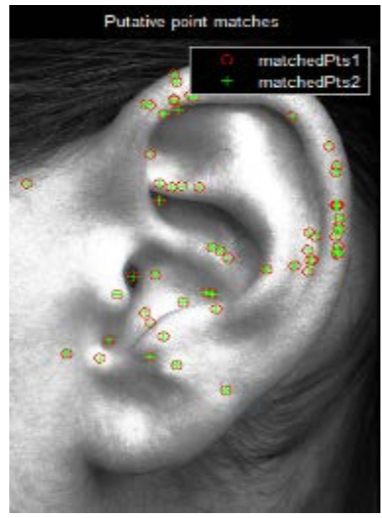
\includegraphics[width=0.5\textwidth]{Figures/Figure15}
	\end{center}
	\caption{The matching results of SURF detector}
	\label{fig:Figure15}
\end{figure}

\begin{figure}[t]
	\DeclareGraphicsExtensions{.pdf,.png,.jpg}
	\begin{center}
		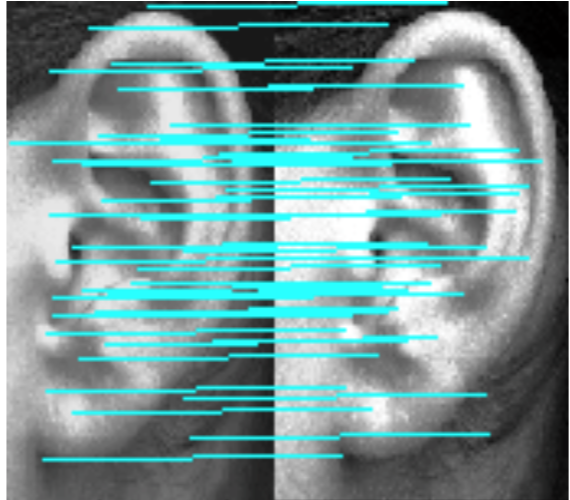
\includegraphics[width=0.5\textwidth]{Figures/Figure16}
	\end{center}
	\caption{The matching results of SIFT detector}
	\label{fig:Figure16}
\end{figure}


\begin{figure}[b]
	\DeclareGraphicsExtensions{.pdf,.png,.jpg}
	\begin{center}
		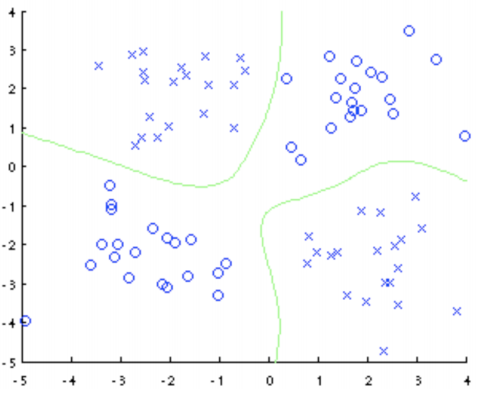
\includegraphics[width=0.5\textwidth]{Figures/Figure10}
	\end{center}
	\caption{Multi-class SVM(from [libSVM paper])}
	\label{fig:Figure10}
\end{figure}

Support Vector Machines(SVMs)\cite{vapnik} brought a completely new idea to the field of machine learning. SVMs were introduced in COLT-92 by Boser,Guyon and Vapnik. For Pattern Recognition, SVMs have been used for Handwriting Recognition, Object Recognition, speaker identification, charmed quark detection, text categorization, face detection in images and many other purposes. SVMs are supervised learning models, with learning algorithms which are associated with it which are used to analyze data for classification and regression purposes. Given a set of training examples, each marked for belonging to one of two categories, an SVM training algorithm builds a model that assigns new examples into one category or the other, making it a non-probabilistic binary linear classifier. An SVM model is a representation of the examples as points in space, mapped so that the examples of the separate categories are divided by a clear gap that is as wide as possible. New examples are then mapped into that same space and predicted to belong to a category based on which side of the gap they fall on.

In addition to performing linear classification, SVMs can efficiently perform a non-linear classification using what is called the kernel trick, implicitly mapping their inputs into high-dimensional feature spaces.When data are not labeled, a supervised learning is not possible, and an unsupervised learning is required, that would find natural clustering of the data to groups, and map new data to these formed groups. The clustering algorithm which provides an improvement to the support vector machines is called support vector clustering and is often used in industrial applications either when data is not labeled or when only some data is labeled as a preprocessing for a classification pass.

SVMs can be divided into linear SVM and multi-class SVM, here we are more concerned with mulit-class SVM\cite{multiSVM}.

For our purpose we have used Multi-class SVMs. Support Vector Machines were originally designed for binary classification. The formulation to solve Multi-class SVM must have variables which are proportional to the number of different classes. The concept of SVM was proposed by Vapnik  et al. They helped to classify almost everything right from linear problems to multi-dimensional problems where the kernel matrix is use to transform the conflicting points into a different dimensional space called the kernel space in order to draw a hyperplane in a conclusive manner so as to separate the different cases. Here multiclass SVM is being used in order to classify the features as extracted by the various feature extraction techniques like SURF and SIFT. After that the model is trained and the features are matched with the features obtained from the query ear image in order to find a nearest match to succeed. Since it is multi-class, thus it helps to create separate classes for different classes of images and helps to classify them when the matching process is being done. The main process of better classification of the model depends on the input features. So as a matter of fact we can say that better the feature extraction is being done, better will be the classification made by the multiclass SVM and thus better will be the results.

The Results can be found in the next section.


\section{Results of the Traditional Approach}
The proposed approach has been evaluated on two data sets. One is the AMI database \cite{AMI}, which consists of 175 ear images; and the other is the IIT Delhi database \cite{IIT}, which consists of 494 images of 125 distinct persons. The images were all converted to gray- scale images for ease of work. It has also been found out that contrast enhancement is an important factor for feature detection and matching, because it makes the feature detectors find better set of keypoints and increase the effectiveness of matching.
According to the experiments performed, it has been found that upper helix, antihe- lix, and tragus are the most important regions for feature selection compared to others. These regions contribute to about 64{\%} of the feature points.
Figure 7 shows some sample images from the two databases we used for our exper- iments. The graphs in Figure 8 indicates the average number of keypoints found and matched by SIFT and SURF detectors when the images are rotated from a range of 0 to 180 degrees. The results suggest that the SIFT detector is fairly stable over a variation of angles from 20 to 160 degrees, whereas the SURF detector, though faster and rotation invariant, is not very stable.
Table 1 shows the keypoints detected and matched by the SIFT and SURF detectors, where the performance ratio is the ratio of the number of matched points to that of detected features. It is obvious that the SIFT algorithm performs better when the sizes of images are decreased, while the SURF algorithm performs better when the image sizes are increased. However, the amount of detected keypoints by the SIFT detector is always higher than that by the SURF detector.

\begin{table}[]
\centering
\caption{SIFT and SURF detection and matching results at different scales}
\label{table1}
\begin{tabular}{lllllllllll}
\hline
\multicolumn{1}{c}{Scaling} &           
\multicolumn{1}{c}{Methods} &          
\multicolumn{1}{c}{0.25} &     
\multicolumn{1}{c}{0.5} &     
\multicolumn{1}{c}{0.75} &     
\multicolumn{1}{c}{1.0} &     
\multicolumn{1}{c}{2.0} &     
\multicolumn{1}{c}{3.0} &     
\multicolumn{1}{c}{4.0} &       \\ \cline{1-2}
\hline
 Number of Features & SIFT  & 28  & 53  & 58 & 64 & 170  & 247  & 233   \\
 & SURF & 3  & 12  & 30 & 41 & 39 & 41 & 44   \\
 \hline
  Number of Matches & SIFT  & 24  & 45  & 54 & 64 & 53  & 47  & 51   \\
 & SURF & 2  & 9  & 23 & 41 & 20 & 21 & 16   \\
 \hline
 Performance Ratio & SIFT  & 0.85  & .85  & 0.89 & 1.0 & 0.32 & .20 & 0.22  \\
 & SURF & 0.67 & 0.75  & 0.75 & 1.0  &  0.51 & 0.51 & .30  \\
 \hline
\end{tabular}
\end{table}

\begin{table}[]
\centering
\caption{Experimental results on the IIT Delhi database}
\label{table2}
\begin{tabular}{lllllll}
\hline
\multicolumn{1}{c}{Method} &           
\multicolumn{1}{c}{Number of Images} &          
\multicolumn{1}{c}{Matched } &     
\multicolumn{1}{c}{Unmatched } &     
\multicolumn{1}{c}{Time} &     
\multicolumn{1}{c}{Recognition Rate} &     \\ \cline{1-2}
\hline
SIFT  & 125  & 121  & 4 & 0.21 & 96.8 {\%}  \\
\hline
SURF & 125  & 118  & 7 & 0.183 & 94.4 {\%}    \\
 \hline

\end{tabular}
\end{table}

Table 2 shows an overview of how the two detectors work in real-life conditions where some images are not matched due to illumination changes as those images were mostly taken at night and at different angles. Thus, the descriptors fail to find enough feature keypoints for matching. The overall recognition rates of the SIFT and SURF algorithms on the IIT Delhi database are 96.8{\%}and 94.4{\%}, respectively. As a comparison, we also implemented other methods for ear recognition. The template matching technique yields a recognition rate of 93 {\%} for \cite{ansari}, and 92.6 {\%} for \cite{birbhanu}, whereas the recognition rate by the contour extraction technique \cite{bowyer} is 85 {\%} It is evident that the proposed technique yields a higher recognition rate.

\begin{table}[]
\centering
\caption{Einal Results after the outlier detection}
\label{table3}
\begin{tabular}{llllll}
\hline
\multicolumn{1}{c}{Method} &           
\multicolumn{1}{c}{Number of Images} &          
\multicolumn{1}{c}{Matched } &     
\multicolumn{1}{c}{Unmatched } &        
\multicolumn{1}{c}{Recognition Rate} &     \\ \cline{1-2}
\hline
SIFT  & 125  & 119  & 6  & 95.2 {\%}  \\
\hline
SURF & 125  & 114  & 11  & 91.2 {\%}    \\
 \hline

\end{tabular}
\end{table}

From the above table \ref{table3}, it can be seen that due the removal of outliers - the number of false matches have decreased to a certain extent. Thus, the false matches have been successfully removed keeping in mind that the noise in the image is gaussian, the performance of the algorithm decreases but the algorithm is robust and thus is more favourable than the previous approach.

\begin{figure}
	\DeclareGraphicsExtensions{.pdf,.png,.jpg}
		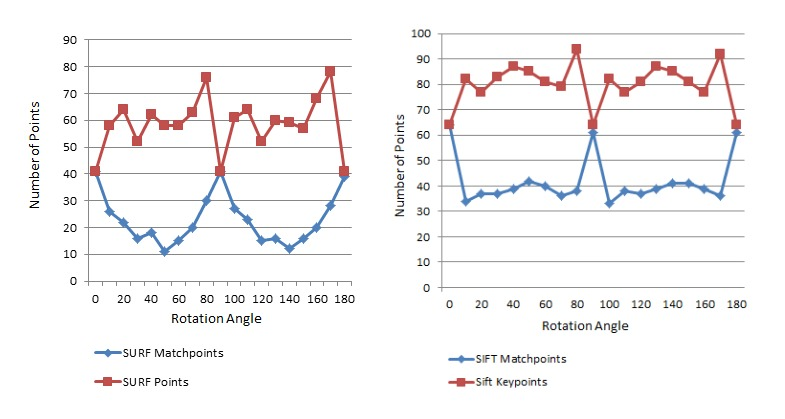
\includegraphics[width=\textwidth]{Figures/Figure17}
	\caption{A comparison result of the detected and matched keypoints by SURF and SIFT}
	\label{fig:Figure13}
\end{figure}

\begin{figure}
	\DeclareGraphicsExtensions{.pdf,.png,.jpg}
	\begin{center}
		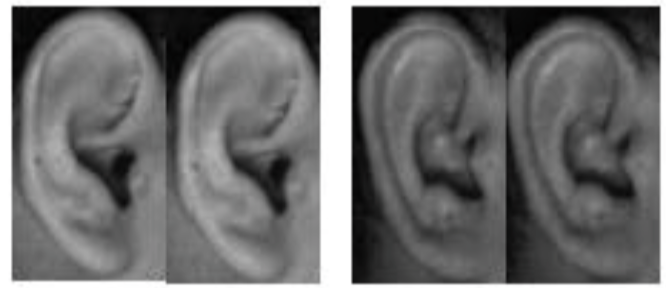
\includegraphics[width=0.5\textwidth]{Figures/Figure13}
	\end{center}
	\caption{Sample Images from IIT Delhi Ear Dataset}
	\label{fig:Figure13}
\end{figure}

\begin{figure}
	\DeclareGraphicsExtensions{.pdf,.png,.jpg}
	\begin{center}
		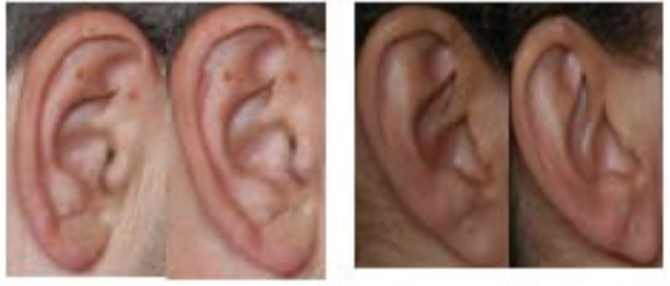
\includegraphics[width=0.5\textwidth]{Figures/Figure14}
	\end{center}
	\caption{Sample Images from AMI Ear Dataset}
	\label{fig:Figure14}
\end{figure}
\chapter{Improved Deep Design}

\section{Deep Learning Approach} \label{sec:build4}

Artificial Neural Networks shown in Figure \ref{fig:Figure20} was an idea conceived  in the 1960s to mimic the functions of the human brain in the way it absorbs information and learns from it. in order to  convert the whole notion into reality it took a lot more time than expected. The primary reason behind the delay is that back then, the computers were not powerful enough, the other reasons being the researchers were not totally aware of the problem. Then in 1986, eminent neural network researcher and computer scientist Dr. Geoffrey Hinton came up with the idea of backpropagation[hinton paper] where a Deep Neural Network could be trained discriminatively and the weight updates can be done via stochastic gradient descentusing the following equation.

\begin{center}
	$w_{ij}(t+1) = w_{ij}(t) + \eta \frac{\partial C}{\partial w_{ij}}$
\end{center}
where $\eta$ s the learning rate, C is the cost function. The choice of the cost function depends on factors such as learning type whether it be supervised, unsupervised or reinforcement learning. 

\begin{figure}[t]
	\DeclareGraphicsExtensions{.pdf,.png,.jpg}
	\begin{center}
		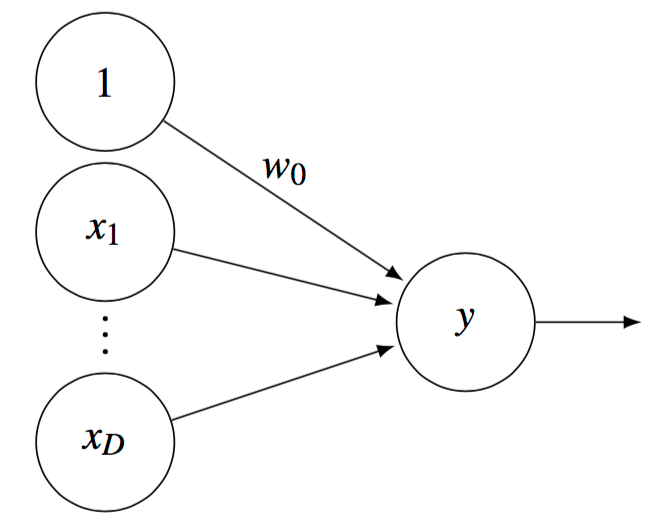
\includegraphics[width=0.7\textwidth]{Figures/Figure20}
	\end{center}
	\caption{Artificial Neural Network with D input neurons and 1 output neuron} 
	\label{fig:Figure20}
\end{figure}


The ability of multi-layer backpropagation[hinton backpropagation paper] networks has enabled the machines to learn complex high-dimensional non-linear mappings from large collections of example data which makes it obvious for visual recognition. In this method, rather than hand-crafting the various features, a raw image is first convoluted with a filter to find various feature maps. The feature maps are then connected together to form a fully-connected layer, the input of one layer is fed as the output of the next layer to create a deep network. The whole process rely on backpropagation to turn the first few layers into an appropriate feature extractor. Deep learning has achieved a lot of successes in the past for character recognition, digit recognition and recent works show that it is being applied to most topics of image representation and learning purposes. Just recently it has been applied to Face Recognition by training with lots of face image data and tremendous success has been reported[deep face paper].

The whole process of deep Convolutional Neural Networks(CNN)[leCunn paper] is very complex and requires a lot of computation to train and as a matter of fact, parallel computing is being brought forward to decrease the training time. The fully connected layer has several hundred hidden units and each of these units have specific weights assigned to them with the help of the back-propagation algorithm. Overfitting occurs if training data is scarce. Before being connected to the fully-connected neural network, the images need to be size normalized and centered in input fields. CNNs force the extraction of certain local features rather than global features which are obtained by hand-crafted feature extractors.

Deep Learning research stopped even after all these breakthroughs because the computers took a lot of time to train the large neural nets and at the same time a lot of image data was also not available. Researchers thought that it is better to go ahead with hand-crafted feature extractors which were giving better results at that time and took less time for computation. In 2006, Geoffrey Hinton and Ruslan Salakhuditnov worked on reducing the dimension of the data with neural networks in thier paper[DBN paper]. Since then a lot of work has been done as computers have become powerful with the advent of modern parallel processing algorithms. One of the major breakthroughs came in 2012, when Alex Krizhevsky[AlexNet paper] build a huge neural network by training 15 million images and then using Deep CNN they got one of the best result in the ImageNet competition for Image recognition and got a result which  was nearly 11 p.c. better than the second best approach which was done with SIFT + Fisher Vectors [Fei Fei Li paper]. Since then in the last 4 years quite a good amount of work has been done in this field. Several deep learning frameworks have been designed by researchers for researchers to move the work ahead - Some of the famous Frameworks being Caffe[Caffe Paper] by University of California, Berkeley, Theano[Theano Paper] by University de Montreal, TensorFlow[TF Paper] by Google, Torch[Torch Paper] and many others.

In our project we have used the Caffe Deep Learning Framework[Caffe Paper] for our purposes. The reason we choose Caffe is being described below:

Caffe provides multimedia scientists and practitioners with a clean and modifiable framework for state of the art deep learning algorithms. It has a big collection of reference CNN models, it is licensed with BSD and is written in C++ and Python. Caffe can process upto 40 million images a day on a single NVIDIA K40. Caffe is maintained by Berkeley Vision and Learning Center(BVLC). Caffe makes it easy for users to build CNNs in their .prototxt file and also has several functions to draw networks and optimize them. It provides Pre-Trained models which is not provided by many of its competetitors. Caffe stores nd communicates data in 4-arrays called blobs for faster processing. Blobs provide a unified memory interface, holding batches of images , parameters or parameters updates. Blobs conceal the mental and mental overhead of mixed CPU/GPU operation by synchronizing from the CPU host to the CPU device as needed. 

A key problem in multimedia data analysis is discovery of effective representations for sensory inputs—images, sound- waves, haptics, etc. While performance of conventional, handcrafted features has plateaued in recent years, new developments in deep compositional architectures have kept performance levels rising [8:caffe paper]. Deep models have outper- formed hand-engineered feature representations in many do- mains, and made learning possible in domains where engi- neered features were lacking entirely.
We are particularly motivated by large-scale visual recog- nition, where a specific type of deep architecture has achieved a commanding lead on the state-of-the-art. These Con- volutional Neural Networks, or CNNs, are discriminatively trained via back-propagation through layers of convolutional filters and other operations such as rectification and pooling. Following the early success of digit classification in the 90’s, these models have recently surpassed all known methods for large-scale visual recognition, and have been adopted by in- dustry heavyweights such as Google, Facebook, and Baidu for image understanding and search.

While deep neural networks have attracted enthusiastic interest within computer vision and beyond, replication of published results can involve months of work by a researcher or engineer. Sometimes researchers deem it worthwhile to release trained models along with the paper advertising their performance. But trained models alone are not sufficient for rapid research progress and emerging commercial applications, and few toolboxes offer truly off-the-shelf deployment of state-of-the-art models—and those that do are often not computationally efficient and thus unsuitable for commercial deployment.

Caffe has several advantages over its peers. Caffe provides a complete toolkit for training, testing, finetuning, and deploying models, with well-documented examples for all of these tasks. As such, it’s an ideal starting point for researchers and other developers looking to jump into state-of-the-art machine learning. At the same time, it’s likely the fastest available implementation of these algorithms, making it immediately useful for industrial deployment.

Some of the main features of Caffe are:\\
\textbf{Modularity:} The software is designed from the begin- ning to be as modular as possible, allowing easy extension to new data formats, network layers, and loss functions. Lots of layers and loss functions are already implemented, and plentiful examples show how these are composed into train- able recognition systems for various tasks. \\

 \textbf{Separation of representation and implementation:} Caffe model definitions are written as config files using the Protocol Buffer language. Caffe supports network archi- tectures in the form of arbitrary directed acyclic graphs. Upon instantiation, Caffe reserves exactly as much memory as needed for the network, and abstracts from its underly- ing location in host or GPU. Switching between a CPU and GPU implementation is exactly one function call. \\

\textbf{Test coverage:} Every single module in Caffe has a test, and no new code is accepted into the project without corre- sponding tests. This allows rapid improvements and refac- toring of the codebase, and imparts a welcome feeling of peacefulness to the researchers using the code. \\

\textbf{Python and MATLAB bindings:} For rapid proto- typing and interfacing with existing research code, Caffe provides Python and MATLAB bindings. Both languages may be used to construct networks and classify inputs. The Python bindings also expose the solver module for easy pro- totyping of new training procedures.

Caffe Neural Network Model prototxt format is being shown below:

\begin{lstlisting}% Start your code-block
name: "LeNet"
layer {
  name: "data"
  type: "Input"
  top: "data"
  input_param { shape: { dim: 64 dim: 1 dim: 28 dim: 28 } }
}
layer {
  name: "conv1"
  type: "Convolution"
  bottom: "data"
  top: "conv1"
  param {
    lr_mult: 1
  }
  param {
    lr_mult: 2
  }
  convolution_param {
    num_output: 20
    kernel_size: 5
    stride: 1
    weight_filler {
      type: "xavier"
    }
    bias_filler {
      type: "constant"
    }
  }
}
layer {
  name: "pool1"
  type: "Pooling"
  bottom: "conv1"
  top: "pool1"
  pooling_param {
    pool: MAX
    kernel_size: 2
    stride: 2
  }
}
layer {
  name: "conv2"
  type: "Convolution"
  bottom: "pool1"
  top: "conv2"
  param {
    lr_mult: 1
  }
  param {
    lr_mult: 2
  }
  convolution_param {
    num_output: 50
    kernel_size: 5
    stride: 1
    weight_filler {
      type: "xavier"
    }
    bias_filler {
      type: "constant"
    }
  }
}
layer {
  name: "pool2"
  type: "Pooling"
  bottom: "conv2"
  top: "pool2"
  pooling_param {
    pool: MAX
    kernel_size: 2
    stride: 2
  }
}
layer {
  name: "ip1"
  type: "InnerProduct"
  bottom: "pool2"
  top: "ip1"
  param {
    lr_mult: 1
  }
  param {
    lr_mult: 2
  }
  inner_product_param {
    num_output: 500
    weight_filler {
      type: "xavier"
    }
    bias_filler {
      type: "constant"
    }
  }
}
layer {
  name: "relu1"
  type: "ReLU"
  bottom: "ip1"
  top: "ip1"
}
layer {
  name: "ip2"
  type: "InnerProduct"
  bottom: "ip1"
  top: "ip2"
  param {
    lr_mult: 1
  }
  param {
    lr_mult: 2
  }
  inner_product_param {
    num_output: 10
    weight_filler {
      type: "xavier"
    }
    bias_filler {
      type: "constant"
    }
  }
}
layer {
  name: "prob"
  type: "Softmax"
  bottom: "ip2"
  top: "prob"
}
\end{lstlisting}

\begin{figure}[t]
	\DeclareGraphicsExtensions{.pdf,.png,.jpg}
	\begin{center}
		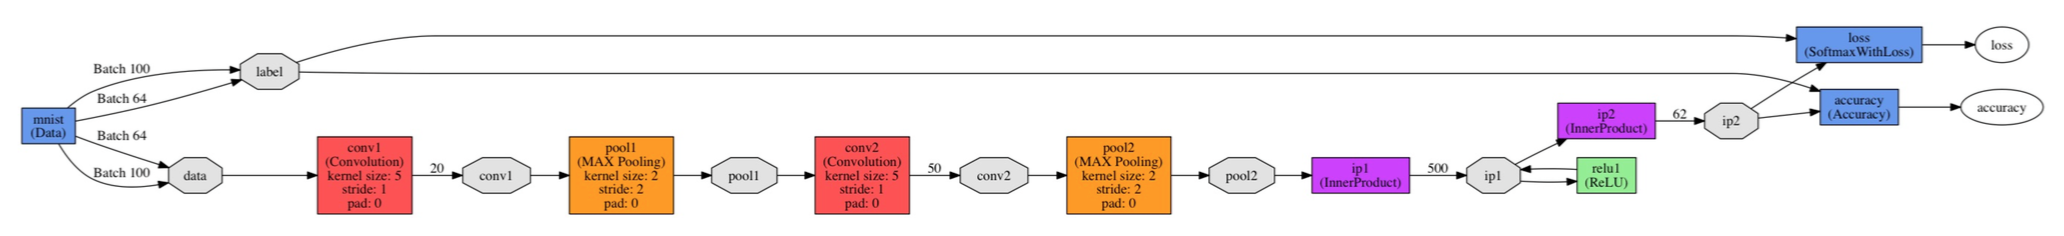
\includegraphics[width=\textwidth]{Figures/Figure18}
	\end{center}
	\caption{LeNet Network Diagram}
	\label{fig:Figure18}
\end{figure}

\section{Convolution Neural Network} \label{sec:build5}

Convolution Neural Network [CNN Paper] combine different architectural ideas to ensure  shift and distortion invariances. In the Figure \ref{fig:Figure19} below it  can be seen that the input plane receives images that are approximately size-normalized and centered. Each unit of a layer receives input from units which are located locally in the previous layer. With local fields, it becomes easier for the neurons to extract visual features such as oriented edges, corners etc, these features are then combined by the higher layer called feature maps. It is being stated that distortion or shift in inputs causes the position of the salient features to vary. 

\begin{figure}[t]
	\DeclareGraphicsExtensions{.pdf,.png,.jpg}
	\begin{center}
		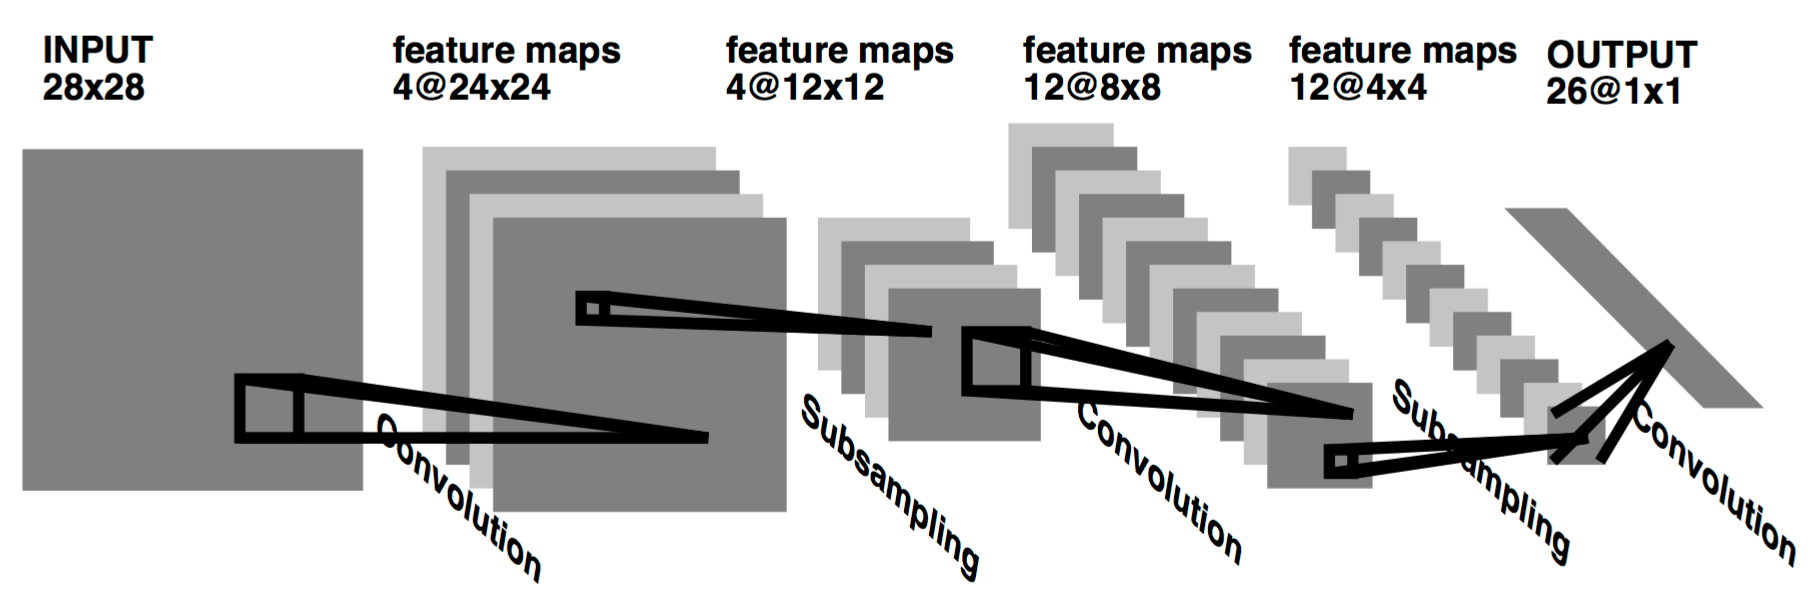
\includegraphics[width=\textwidth]{Figures/Figure19}
	\end{center}
	\caption{Typical CNN Network}
	\label{fig:Figure19}
\end{figure}


At each position, different types of units in different feature maps compute different types of features. A convolution layer is usually composed of several feature maps and as a matter of fact multiple features can be extracted at each location. The hidden layer in Figure \ref{fig:Figure19} has 4 feature maps with 5 by 5 receptive fields. Shifting the input of a convolution layer will shift the output. After detecting a feature, its location becomes less important as long as its relative position to other features is preserved. Thus, each convolution layer is followed by an additional layer while is called the pooling layer and it performs the subsampling and local averaging, thereby reducing the resolution of the feature map which reduces the effect to shifts and distortions. The second layer performs a 2 X 2 averaging and subsampling, followed by a trainable coefficient, a trainable bias , and a bias. The trainable coefficient and bias controls the effect of non-linearity. Then alternating layers of subsampling and convolutions are created successively where at each layer the number of feature maps are increased but the spatial resolution is decreased. The feature maps are then connected to form a fully-connected layer which is being fed into the softmax regression layer for classification purposes. All the weights are learned in the respective layers with back-propagation.

In recent times, Convolution Neural Networks(CNNs) have almost been used in all applications ranging from the popular ImageNet Large Scale Visual Recognition Challenge(ILSVRC) to various Recognition algorithms. It has taken the computer vision society by storm, improving the state of the art in many applications. Tremendous results have been obtained in tremendous large scale databases in recent times. \\

\textbf{ReLU Non-Linearity - } In CNNs, the standard way to model a neuron's output f as a function of of its input \textit{x} is with \textit{f(x) = tanh(x)} or \textit{f(x) = $(1+e^{-x})^{-1}$} . The training time with gradient descent algorithm is much slower due to saturation and nonlinearities thus a new concept can be applied here with non saturating neurons with nonlinearities where \textit{f(x) = max(0,x)}. These nuerons are known as Rectified Linear Units(ReLUs). CNNs with ReLUs train muc faster than their corresponding tanh units. The performance of the neurons also doesnot decrease as proven with experiments by Hinton and Nair[Hinton and Nair paper]. 

\begin{figure}
	\DeclareGraphicsExtensions{.pdf,.png,.jpg}
	\begin{center}
		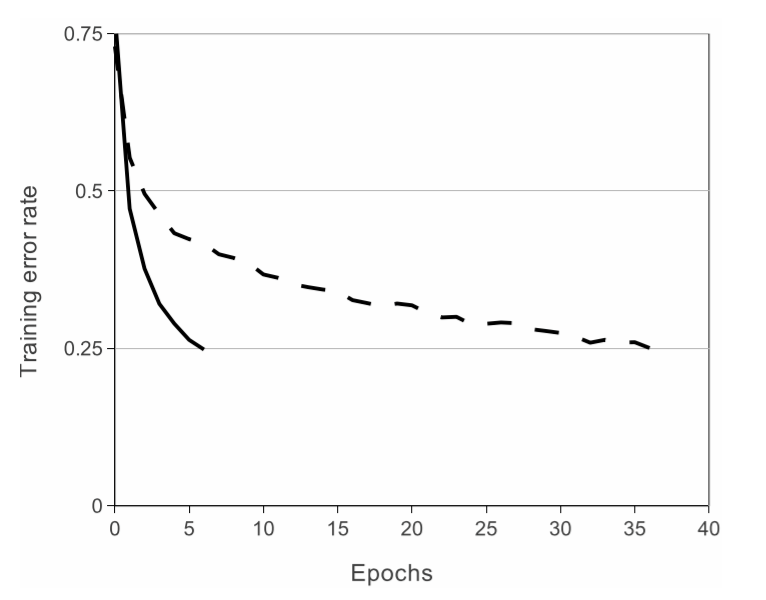
\includegraphics[width=0.5\textwidth]{Figures/Figure21}
	\end{center}
	\caption{Performance of a 4-layer ReLU CNN}
	\label{fig:Figure21}
\end{figure}

Figure \ref{fig:Figure21} [AlexNet paper] shows the number of iterations required to reach 25 p.c. training error on the CIFAR-10 dataset for a four layer convolution network. Thus it can be shown that faster learning has a great influence on the performance of large models which are trained on large datasets.

Another important concept to reduce test errors is the dropout technique. It seems to be too expensive for the big CNNs to train, which take several days to complete even on GPUs. The dropout technique consists of setting to zero the output of each hidden neuron with 50 p.c. probability, the dropped out neurons do not contribute to the forward pass and also do not participate in back-propagation approach. So every time, the neural network samples a different architecture but all the architecture share weights. This technique educes the complex o-adaptations of neurons since a neuron cannot rely on the presence of particular other neurons.It is, therefore, forced to learn more robust features that are useful in conjunction with many different random subsets of the other neurons. At test time, we use all the neurons but multiply their outputs by 0.5, which is a reasonable approximation to taking the geometric mean of the predictive distributions produced by the exponentially-many dropout networks.

Dropout is mostly applied to the Fully-connected layer in a CNN. Dropout helps to prevent overfitting in a neural networknd thus is an extremely useful concept.




\section{Our Deep Network and Model} \label{sec:build6}
\section{Results of the Deep Approach}
\label{sec:results2}

Synthesis of the second redesign of the scheduler module targeting a Xilinx
\cite{xilinx} Virtex-II Pro 30 yields the following FPGA resource statistics:
1,034 out of 13,696 slices, 522 out of 27,392 slice flip-flops, 1,900 out of
27,392 4-input LUTs, and 2 out of 136 BRAMs.  The module has a maximum
operating frequency of 143.8 MHz, which easily meets our goal of a 100 MHz
clock frequency.


\chapter{Conclusion} \label{sec:conc} In this project we have studied two scale and rotation invariant feature detecters and their application to ear recognition. Although both the SIFT and the SURF are invariant under scale and rotation changes, their performance decreases under certain conditions. The SIFT detector is more stable than the SURF detector under rotation changes. It is also found that the SIFT algorithm performs better for image decreasing, in contrast, the SURF algorithm performs better for image increasing.False matches have always caused problem for researchers in this field and it hinders the performance of the systems, thus Robust and Fast algorithm has been implemented to remove potential false matches and get better results. Experimental evaluations have demonstrated the effectiveness of the proposed techniques in ear recognition. For future work, an ear dataset consisting of thousands to millions of images must be created and preprocessed for better performances. Work must be done with the help of deep learning algorithms, which must be able to extract features automatically from less training data and as a matter of fact it would make it easier to train on CPUs and also give better performances.

Deep Learning models can be used for various purposes and thus the models must be applied to other biometric datasets to compare their performances. As of now, deep learning has mostly been applied to face recognition algorithms and has received tremendous success, thus work must be done on other sets of biometrics like iris, fingerprint, palm and others for better performances.


%\section*{Acknowledgment}


\medskip

\bibliographystyle{ieeetr}
\bibliography{ref1}

\chapter{Appendix}
\label{sec:A}
\textbf{1. Code for Robust Fundamental Matrix}
\begin{lstlisting}

function [F,inliers] =RobustFundaMatrix(x1,x2)
numpts=size(x1,2);
[Fi,e1i,e2i]=fundmatrix(x1,x2);
Pai=eye(3,4);Pbi = vgg_P_from_F(Fi);
Xe=zeros(4,numpts);
err=zeros(1,numpts);
et=err;
for i=1:numpts
    Xe(:,i)=optimalTriangulation(x1(:,i),x2(:,i),Pai,Pbi,Fi,e1i,e2i);
    err(i)=sqrt(norm(pflat(Pai*Xe(:,i))-x1(:,i))^2+
    norm(pflat(Pbi*Xe(:,i))-x2(:,i))^2);
    et(i)=sum(pflat(Pai*Xe(:,i))-x1(:,i))+
    sum(pflat(Pbi*Xe(:,i))-x2(:,i));
end
m=median(abs(err));
sigma=1.4826*(1+5/(numpts-8))*m;
index=find(abs(err)<3*sigma);
[F,e1,e2]=fundmatrix(x1(:,index),x2(:,index));
Pa=eye(3,4);Pb = vgg_P_from_F(F);
for i=1:numpts
    Xe(:,i)=optimalTriangulation(x1(:,i),x2(:,i),Pa,Pb,F,e1,e2);        
    err(i)=sqrt(norm(pflat(Pa*Xe(:,i))-x1(:,i))^2+
    norm(pflat(Pb*Xe(:,i))-x2(:,i))^2);
    et(i)=sum(pflat(Pai*Xe(:,i))-x1(:,i))+
    sum(pflat(Pbi*Xe(:,i))-x2(:,i));
end
m=median(abs(err));
sigma=1.4826*(1+5/(numpts-8))*m;
index=find(abs(err)<3*sigma);
F=fundmatrix(x1(:,index),x2(:,index));
inliers=index;

\end{lstlisting}

\label{sec:B}
\textbf{2. Code for Optimal Triangulation}

\begin{lstlisting}

function  X  = optimalTriangulation( x1,x2,P1,P2,F,e1,e2 )
% [ X,r ] = optimalTriangulation( x1,x2,P1,P2,F,e1,e2 )
%   Optimal solution for MLE, using method proposed by Hartley(P315).
%   Finding optimal solution by finding real solutions of a polynomial 
equation of degree  6.
%   

if any(size(x1)~=size(x2))
    error('size(x1)~=size(x2)');
end

if size(x1,1)==2  % convert x1,x2 to form of (x,y,1)
    x1=[x1;1];
    x2=[x2;1];
else
    x1(1)=x1(1)./x1(3);x1(2)=x1(2)./x1(3);x1(3)=1;
    x2(1)=x2(1)./x2(3);x2(2)=x2(2)./x2(3);x2(3)=1;
end

T1=[1 0 -x1(1);0 1 -x1(2);0 0 1];T1_inv=[1 0 x1(1);0 1 x1(2);0 0 1];
T2=[1 0 -x2(1);0 1 -x2(2);0 0 1];T2_inv=[1 0 x2(1);0 1 x2(2);0 0 1];
F=T2_inv.'*F*T1_inv;
%x1=[0;0;1];%T1*x1;
%x2=[0;0;1];%T2*x2;
e1=T1*e1;e1=e1/norm(e1(1:2));
e2=T2*e2;e2=e2/norm(e2(1:2));
R1=[e1(1) e1(2) 0;-e1(2) e1(1) 0;0 0 1];
R2=[e2(1) e2(2) 0;-e2(2) e2(1) 0;0 0 1];
%e1=[1;0;e1(3)];%R1*e1;
%e2=[1;0;e2(3)];%R2*e2;
F=R2*F*R1.';
f1=e1(3);f2=e2(3);a=F(2,2);b=F(2,3);c=F(3,2);d=F(3,3);
%F_=[f1*f2*d -f2*c -f2*d;-f1*b a b;-f1*d c d];
%F./F_


f1_2=f1^2;f1_4=f1_2^2;f2_2=f2^2;
k1=a^2+f2_2*c^2;k2=2*(a*b+f2_2*c*d);k3=b^2+f2_2*d^2;
k=a*d-b*c;k4=a*c;k5=b*c+a*d;k6=b*d;
c6=-f1_4*k*k4;
c5=k1^2 - f1_4*k*k5;
c4=2*k1*k2 - 2*f1_2*k*k4 - f1_4*k*k6;
c3=k2^2 + 2*k1*k3 - 2*f1_2*k*k5;
c2=2*k2*k3 - k*k4 - 2*f1_2*k*k6;
c1=k3^2 - k*k5;
c0=- k*k6;
% Threshold to set some very samll cis to 0.
p=[c6 c5 c4 c3 c2 c1 c0];
Mci=max(abs(p));
for i=1:6
    if abs(p(i))<Mci*1e-25  % threshold ratio is chosen to be 1e-20
        p(i)=0;
    end
end
if sum(isnan(p))~=0 || sum(isinf(p))~=0
    X=zeros(4,1);return
end
rs=real(roots(p));
nrs=size(rs,1);% number of roots.
s=zeros(nrs+1,1);
for i=1:nrs
    t=rs(i);
    t2=t^2;
    k1_=(a*t+b)^2;
    k2_=(c*t+d)^2;
    s(i)=t2/(1+f1_2*t2)+k2_/(k1_+f2_2*k2_);
end
s(nrs+1)=1/f1_2+c^2/(a^2+f2_2*c^2);
[m I]=min(s);
if I==nrs+1
    l1=[f1;0;-1];
    l2=[-c*f2;a;c];
else
    t=rs(I);
    l1=[t*f1;1;-t];
    l2=[-f2*(c*t+d);a*t+b;c*t+d];
end
x1_=[-l1(1)*l1(3);-l1(2)*l1(3);l1(1)^2+l1(2)^2];
x2_=[-l2(1)*l2(3);-l2(2)*l2(3);l2(1)^2+l2(2)^2];
%r=sqrt((x1_(1)^2+x1_(2)^2)/x1_(3)^2+(x2_(1)^2+x2_(2)^2)/x2_(3)^2);
% residual
%r=sqrt(m);
x1_=T1_inv*R1.'*x1_;
x2_=T2_inv*R2.'*x2_;

Ax=zeros(4,4);
Ax(1,:)=x1_(1)*P1(3,:)-x1_(3)*P1(1,:);
Ax(2,:)=x1_(2)*P1(3,:)-x1_(3)*P1(2,:);
Ax(3,:)=x2_(1)*P2(3,:)-x2_(3)*P2(1,:);
Ax(4,:)=x2_(2)*P2(3,:)-x2_(3)*P2(2,:);
[u s v]=svd(Ax);
X=v(:,end);

end



\end{lstlisting}

\label{sec:C}
\textbf{3.Basic Code for SIFT Matching }
\begin{lstlisting}

 [image1,descrips,locs]=sift('ear1.pgm');
% You cannot change the name of the locs, that is why,it is 
being stored in
% loc1 for later use
locs1=locs;%loc1 is locs for first first image,same with loc2
and descrips1 and descrips 2.
descrips1=descrips;
[image2,descrips,locs]=sift('ear1.pgm');
locs2=locs;
descrips2=descrips;
[num,matches] = match(image1,descrips1,locs1,image2,descrips2,locs2);
if num<5
    fprintf('Match Failed')
    title('Match Failed')
    return
end
x1=[loc1(matches(1,:),1:2),ones(size(matches,2),1)]';
x2=[loc2(matches(2,:),1:2),ones(size(matches,2),1)]';
[F,inliers]=RobustFundaMatrix(x1,x2);
threshold=0.7;
if length(inliers)/size(matches,2)>threshold
    result=1;
    fprintf('Match');
    title('Match')
else
    result=0;
    fprintf('Failed');
    title('Failed');
end

\end{lstlisting}

\label{sec:D}
\textbf{4.Basic Code for SURF Feature extraction}
\begin{lstlisting}

I1 = imread('ear1.pgm');
I2 = imread('ear2.pgm');
points1 = detectSURFFeatures(I1);
points2 = detectSURFFeatures(I2);
[f1, vpts1] = extractFeatures(I1, points1);
[f2, vpts2] = extractFeatures(I2, points2);
index_pairs = matchFeatures(f1, f2) ;
matched_pts1 = vpts1(index_pairs(:, 1));
matched_pts2 = vpts2(index_pairs(:, 2));
figure, showMatchedFeatures(I1,I2,matched_pts1,matched_pts2);
title('Putative point matches');
legend('matchedPts1','matchedPts2');

\end{lstlisting}

\end{document}
